% !TEX root = paper.tex
% Contact  jshin@csie.ncnu.edu.tw or pkoehn@inf.ed.ac.uk
%%
%% Based on the style files for ACL-IJCNLP-2009, which were, in turn,
%% based on the style files for EACL-2009 and IJCNLP-2008...

%% Based on the style files for EACL 2006 by 
%%e.agirre@ehu.es or Sergi.Balari@uab.es
%% and that of ACL 08 by Joakim Nivre and Noah Smith

\documentclass[11pt]{article}
\usepackage{latex/acl2010}
\usepackage{times}
\usepackage{url}
\usepackage{latexsym}
%\setlength\titlebox{6.5cm}    % You can expand the title box if you
% really have to

\title{Humuhumunukunukuapua'a}

\author{David Pfau\\
	 \And
  Nicholas Bartlett \\
  Columbia University \\
  New York, NY, United States\\
  {\tt \{dbp2112@, bartlett@stat., fwood@stat.\}columbia.edu}\And
  Frank Wood\\}

\date{}

\begin{document}

\maketitle

% !TEX root = ContextualTopicModel.tex
\begin{abstract}
In this work we describe and test a novel multi-domain, smoothing $n$-gram language model in which the domain from which each word arises is treated as a latent, unknown random variable.  Given the domain for each word, a document is modeled as a sequence of conditional draws (conditioned on the previous words) from a set of domain specific, hierarchically coupled, smoothing $n$-gram language models.  We derive a Bayesian inference procedure for this model and show improved language modeling results in terms of perplexity.
\end{abstract}

% !TEX root = paper.tex
\section{Introduction}

%An image contains many categories of objects.  A song can draw influences from many genres.  And an article may cover many topics within it.  The goal of topic modeling is to extract these latent categories directly from the data, in an unsupervised fashion.  Most topic models ignore the temporal structure of data, treating individual items in a document as exchangeable.  Thus in the case of text modeling, a document is equivalent to a "bag of words."  This is a good approximation of how semantic information is distributed in a document, with associated words appearing throughout a document.  Syntactic information, on the other hand, is intimately tied to word order.  Moreover, topic identities that are ambiguous without context become clear when context is known: the word "states" in "The United States" clearly falls into a different topic than in "altered mental states."  

Generative models for natural language text come in many flavors.  Amongst the most widely used and empirically successful are those that  generate the next word in a sequence from conditional probability tables indexed by a recent subsequence of the preceding words.  This class of generative models includes $n$-gram models  and smoothing variants thereof \cite{Kneser1995,MacKay1995a,Chen1998}, including recent Bayesian nonparametric approaches to the same \cite{Teh2006a,Wood2009}.  

The continuing success of $n$-gram modeling approaches can be attributed to the flexibility and expressiveness of such models, however, few would argue that $n$-gram models correspond structurally to any naturally plausible generative scheme.   For one, $n$-gram models lack completely any latent process that might conditionally influence production.  For instance there is no explicit notion of latent semantic classes for words nor is there a latent topic process.  Every such latent process that one might propose is simply subsumed by the $n$-gram modeling assumption that all regularity and typicality in natural language (grammatical, topic, and otherwise) is captured by local word co-ocurrence patterns.  

%It can be argued models that capture more aspects of the true generative procedure should also do a better job of capturing and modeling typicality.  For instance $n$-gram models are good at representing typicality, but obviously lack parameters and structure that would explicitly encode grammatical rules and the evolution of topics.  
%Sampled sequences from $n$-gram models, both a priori and a posteriori, are not really similar to natural language.  Such sequences are always missing at least two things.  First, the sequences will almost certainly not conform to notions of grammaticality.  Second, there will be little or no topic continuity.  
%Somehow including either or both would undoubtedly result in improvements in both the generative sense and in the model's ability to describe typicality.

%We note here that nominally the ability to distinguish typicality improves as the fidelity of the generative model improves.

There are, of course, many other approaches to language modeling, some of which attempt to address some of these shortcomings.  Tree-based (or parsing) approaches \cite{Roark2001,Collins2003,Johnson2007,Liang2007} to language modeling form a compelling, if not computationally expensive, alternative class of generative models.   %Regardless of whether or not one believes in the innateness of grammar, tree-based generative models, particularly grammars that have been lexicalized in some way, are compelling in that productions from them are at least usually grammatically sensible.  Unfortunately though, like for $n$-gram models, sequences sampled from such models (a priori or a posteriori) also are typically incoherent (just in a different way than the way they are incoherent for $n$-gram models) as they lack even local (intra-sentential) topic coherence.  
Less well known are neural network approaches that make context dependent continuation predictions from large contexts \cite{Mnih2007,Mnih2009}.

%These too have their own  however grammar and parsing based approaches have been partially described in a generative way \cite{Johnson2007,Liang2007}.  Less well known are \cite{Mnih2007,Mnih2009}


In this paper we present a novel natural language model that consists of combining a Bayesian smoothing $n$-gram language model with a topic model.  The point of doing this can either be seen as way of improving $n$-gram language modeling performance or as a way of avoiding the bag of words assumption assumption typical to latent topic models (and correspondingly improving topic modeling performance as well).  The novelty of this work is not in having combined two such models; such combinations have been considered before \cite{Wallach2006}.  Instead, the novelty and contribution here is in the particular choice for each model and in the development of an inference algorithm for the pair.  In prior work, both the specific choice of language model and the way in which that language model was introduced into the topic model effectively limits the order of the $n$-gram language model that can be employed.  In the model we propose here, the depth of the $n$-gram model can easily be extended beyond bi-gram models (the current state of the art), because we make use of a hierarchical language model that shares statistical strength between smoothing $n$-gram language models in a hierarchical Bayesian way \cite{Wood2009}.  
% by introducing document specific topic distributions and per word latent topic indicator variables, in other words introducing a latent topic process.

%In particular we combine Latent Dirichlet Allocation \cite{Blei2003a} and the Doubly-Hierarchical Pitman-Yor Process Language Model \cite{Wood2009}.   an $n$-gram language model which efficiently shares statistical strength between different domains, where in this case a topic constitutes a single domain.  Previous efforts to integrate topic modeling with word order include \cite{Griffiths2005} and \cite{Wallach2006}.  The approach taken by \cite{Griffiths2005} did not allow individual words to play both a semantic and syntactic role.  The approach of \cite{Wallach2006} is similar in spirit to our own, however she uses the hierarchical Dirichlet language model \cite{Mackay1995} which has since been superseded by Bayesian language models with superior performance.  We hope that the use of state-of-the-art language models in topic modeling will lead to both better predictive power and will discover topics that more accurately reflect semantic categories.


\section{Generative Model}

\newcommand{\G}{\mathcal{G}}
\newcommand{\LM}{\mathcal{L}\mathcal{M}}
\newcommand{\bu}{{\bf u}}
\newcommand{\PY}{\mathcal{P}\mathcal{Y}}
\newcommand{\D}{\mathcal{D}}
\newcommand{\LA}{\mathcal{L}}

\subsection{Latent Dirichlet Allocation}

Latent Dirichlet Allocation \cite{Blei and Jordan} is a generative model proposed to model the latent topics present in a set of documents.  If we characterize a topic as a multinomial distribution over words then the generative process can be viewed as treating each document as a mixture of topics. The generative model for $J$ documents containing $T$ possible topics can bes written as 

\begin{eqnarray}
\phi_t | \beta  &\sim& \textrm{Dir}(\beta)  \hspace{1.1cm} t = 1,\ldots,T \nonumber \\
\psi_j | \alpha &\sim& \textrm{Dir}(\alpha) \hspace{1.05cm} j = 1,\ldots, J\nonumber \\
z_{ij} | \psi_j &\sim& \textrm{Mult}(\psi_j) \hspace{.7cm} i = 1,\ldots, N_j \nonumber \\
w_{ij} | \phi_{z_{ij}} &\sim& \textrm{Mult}(\phi_{z_{ij}}) \hspace{.5cm} i = 1,\ldots, N_j 
\end{eqnarray}

where $w_{ij}$ is the $i^{th}$ word in the $j^{th}$ document and $N_j$ is the number of words in document $j$. To generate word $i$ in document $j$ a topic indicator $z_{ij}$ is drawn from the document specific mixture $\psi_j$ and the word is drawn from the appropriate topic $\phi_{z_{ij}}$.  The model may be viewed as a mixed membership model since the words in a document are selected from a mixture of topics.

Efficient estimation of the model can been performed using a collapsed Gibbs sampler \cite{Griffiths2004}.  The parameters $\{ \phi_t \}$ and $\{ \psi_j \}$ are integrated out and each topic label $z_{ij}$ is sampled from the conditional distribution $p(z_{ij} | w_{ij}, \mathbf{z}_{-ij}, \mathbf{w}_{-ij})$.

\subsection{Doubly-Hierarchical Pitman-Yor Process Language Model}

The Doubly-Hierarchical Pitman-Yor Process Language Model (DHPYPLM) \cite{wood and teh} is a nonparametric Bayesian model that ties together individual Hierarchical Pitman-Yor Language Models (HPYPLM). Sharing of statistical strength between language models is achieved through a process known as the Graphical Pitman-Yor Process (GPYP) \cite{wood and teh}.  Because the DHPYPLM builds upon the HPYPLM \cite{teh}, we first describe the HPYPLM.

The HPYPLM is a non-parametric hierarchical Bayesian model specifying that each word is generated from a distribution specific to the context ${\bf u}$ in which the word appears.  For this discussion we will assume that the context of a given word, $w_i$, is the ordered sequence of only the $n-1$ words preceding it, $[w_{i - (n-1)}, w_{i-(n-2)}, \ldots, w_{i-1}]$.  Context specific distributions $\G_{\bu}$ are tied together through the hierarchical structure

\begin{eqnarray}
\G_{[]}| c_0, d_0, \mathcal{U} &\sim& \PY(c_0, d_0, \mathcal{U}) \nonumber \\
\G_\bu | c_{|\bu|}, d_{|\bu|}, \G_{\pi (\bu)} &\sim& \PY( c_{|\bu|}, d_{|\bu|},  \G_{\pi (\bu)}) \label{eqn:hpyplm}
\end{eqnarray}

where $\bu \in \Sigma^{n-1}$, $\Sigma$ is the set of possible words, and $\pi(\bu)$ is the context obtained by removing the most distant word of context $\bu$.  The notation $\G \sim \PY(c,d,\G_0)$ indicates that $\G$ is a random distribution following a Pitman-Yor process \cite{someone} distribution with concentration parameter $c$, discount parameter $d$, and base distribution $\G_0$.

Using of a HPYPLM assumes a single language model responsible for generating all text.  However, there are instances in which the assumption of a single universal language model is inappropriate \cite{Rosenfeld2000}.  In \cite{wood and teh}, using the motivating example of domain adaptation, they suggest the GPYP as a possible solution. The GPYP can be understood as a generative model with a latent, general HPYPLM serving as a common prior for each of several domain specific HPYPLM's.  The common language model is referred to as latent because no data generated directly from the model is ever observed.  Typical of Bayesian hierarchical models, the language model for each domain reflects properties of the general HPYPLM while still capturing differences in the local language structure of each domain.  

In the DHPYPLM, the latent language model is a HPYPLM, as specified by Equation~\ref{eqn:hpyplm}.  If $G^\LA_\bu$ is the distribution over words seen the context $\bu$ in the latent model, then for each domain $\D$,  the domain specific model is

\begin{eqnarray}
\G^\D_{[]} &\sim& \PY(c^\D_0, d^\D_0,\G^\LA_{[]}) \nonumber \\
\G^\D_\bu &\sim& \PY(c^\D_{|\bu|}, c^\D_{|\bu|}, \lambda^\D_{|\bu|}\G^\D_{\pi(\bu)} + (1-\lambda^\D_{|\bu|})\G^\LA_\bu)) \nonumber \\ 
&& \hspace{2cm} \forall \bu \in \Sigma^{n-1}, 0 \leq \lambda^\D_{|\bu|} \leq 1. \nonumber
\end{eqnarray}

Each distribution described is actually a conditional distribution, but the conditioning bars have been left off to de-clutter the notation.  Explicitly, the conditional distribution of $\G^\D_{[]}$ given $c^\D_0, d^\D_0,$ and $\G^\LA_{[]}$, etc.  Note that the base distribution of each Pitman-Yor process for each $\G^\D_\bu$ is a mixture of distributions: the first is the distribution in the same domain given a context shortened by one word while the second is the distribution given the context $\bu$ in the latent language model. Priors are also placed on all $\lambda^\D_{|\bu|}$ parameters, \cite{wood and teh} use

$$\lambda^\D_{|\bu|} \sim \PY(\alpha_{|\bu|}, \delta_{|\bu|}, \textrm{Unif}(0,1))  \hspace{.5cm} \forall \D.$$

Using this prior ties together the $\lambda_{|\bu|}$ parameters across different domains $\D$ under a common prior.

The generative process specified by the  DHPYPLM can be equivalently written in a collapsed representation known as the multi-floor Chinese restaurant franchise (MFCRF) \cite{wood and teh}.  Using the MFCRF \cite{wood and teh} show that estimation can be performed using a collapsed Gibbs sampler.

\subsection{Joining the Models}

We suggest that documents are likely to include language drawn from multiple domains.   Furthermore, we expect local language structure to change across domains. These two hypothesis indicate that an appropriate language model must infer latent domains and a set of language models, tied together through hierarchy, to explain the language structure within a set of documents.

We consider a model which combines the two models previously discussed.  Each document is modeled as a mixture of domains.  To generate the $i^{th}$ word in document $j$, $w_{ij}$, a domain is chosen from the document specific mixture.  Given the domain $z_{ij}$ and the context $\bu$ in which $w_{ij}$ is observed, $w_{ij}$ is drawn from the HPYPLM specific to to domain $z_{ij}$.  The domain specific language models are tied together through the hierarchical structure of the DHPYPLM.  Formally the generative model is

\begin{eqnarray}
\psi_j  &\sim& \textrm{Dir}(\alpha) \nonumber\\
z_{ij}  &\sim& \textrm{Mult}(\psi_j) \nonumber\\
\lambda^{z_{ij}}_{|\bu|} &\sim& \PY(\alpha_{|\bu|}, \delta_{|\bu|}, \textrm{Unif}(0,1)) \nonumber \\
\G^{z_{ij}}_{[]} &\sim& \PY(c^{ z_{ij}}_0, d^{ z_{ij}}_0,\G^\LA_{[]}) \nonumber \\
\G^{ z_{ij}}_\bu &\sim& \PY(c^{ z_{ij}}_{|\bu|}, d^{ z_{ij}}_{|\bu|}, \lambda^{ z_{ij}}_{|\bu|}\G^{ z_{ij}}_{\pi(\bu)} + (1-\lambda^{ z_{ij}}_{|\bu|})\G^\LA_\bu)) \nonumber \\ 
w_{ij}  &\sim& \G^{z_{ij}}_\bu \nonumber.
\end{eqnarray}

The conditioning variables have again been omitted for clarity, but are implicit in the definition.  Figure~\ref{fig:graphicalmodel} shows the graphical model for the proposed model.



\section{Inference}

In the collapsed representation of  the \ourmodel we can estimate the posterior distribution of the parameters using a Gibb's sampler.  The parameters are the vector of topic assignments for each word, ${\bf z}$,  and the set of distributions in the DHPYPLM, which we denote as $\M$.  In the collapsed representation we use for sampling, all the distributions in $\M$ are integrated out, but the predictive distributions needed for sampling are recoverable. The conditional distributions needed to implement a Gibbs sampler are
%
\begin{eqnarray}
& &P(z_{ij} = t | \mathbf{z_{-ij}},\mathbf{w}, \M) \propto  \label{eqn:gibbs1}\\
& &	\hspace{.5cm} P(w_{ij}|z_{ij}=t, \M_{-w_{ij}})P(z_{ij} = t | \mathbf{z}_{-ij}, {\bf w}) \nonumber \\
& &P(\M |  {\bf z} , {\bf w}) \label{eqn:gibbs2} 
\end{eqnarray}
%
\noindent where $\M_{-w_{ij}}$ is a sample from the posterior distribution of the DHPYPLM conditioned on the corpus with the word $w_{ij}$ removed. 

In Equation~\ref{eqn:gibbs1}, $P(w_{ij}|z_{ij}=t, \M_{-w_{ij}})$ is the probability of generating $w_{ij}$ from the language model specific to domain $z_{ij}$ given the current state of the sampler.  This probability is easily calculated given a static state of the DHPYPLM.  The second term in Equation~\ref{eqn:gibbs1} is
%
\begin{eqnarray*}
P(z_{ij} = t | \mathbf{z}_{-ij}, {\bf w}) \propto \frac{n^{(d_j)}_{-ij,t} + \frac{\alpha}{T}}{n^{(d_j)}_{-ij,.} + \alpha},
\end{eqnarray*}
%
\noindent where $n^{(d_j)}_{-ij,t}$ is the number of times the topic $t$ appears in document $d_j$ excluding $w_{ij}$ and the dot indicates marginalization over topics. Equation~\ref{eqn:gibbs2} is the conditional distribution of the DHPYPLM given all the topic assignments.  Sampling from Equation~\ref{eqn:gibbs2} is exactly like the domain adaptation scenario presented in \cite{Wood2009a} and is performed in the multi-floor Chinese restaurant process representation.

\begin{comment}

The term $P(w_{ij}|z_{ij}=t, \mathbf{z}_{-ij}, \mathbf{w}_{-ij})$ in Equation~\ref{eqn:gibbssample} is the probability of generating $w_{ij}$ from the language model specific to domain $z_{ij}$ given the current state of the sampler.  This probability is easily calculated given that the GPYP is sampled in the collapsed MFCRF representation.

Where $n^{(d_j)}_{-ij,t}$ is the number of times the topic $t$ appears in document $d_j$ excluding the token $w_{ij}$, $n^{(w_{ij})}_{-ij,t}$ is the number of times the type $w_{ij}$ appears in topic $t$, excluding the token $w_{ij}$, and the dot represents marginalization (over topics or types).

Posterior inference in the DHPYPLM also takes place via Gibbs sampling.  Rather than representing each draw from a Pitman-Yor process explicitly, we track the clusters to which each observation belongs, as well as the parameter associated with each cluster.  This is a Chinese Restaurant Process representation of a nonparametric model.  Sampling consists of reseating each "customer" within a "restaurant" at a different "table," where an observation is a customer, a restaurant is a draw from a PYP, and a table is a cluster in that draw. In a hierarchical nonparametric model like this, tables in one restaurant are customers in the parent restaurant.  We also place a Gamma(1,1) prior over the concentration parameters and a uniform prior over the discount and switch parameters.  The code for the DHPYPLM was graciously provided by Frank Wood, and the exact details of Gibbs sampling can be found in \ref{Wood2009}.

To integrate the two models, we notice that the second term on the right in equation (2) is independent of our language model and remains unchanged.  The first term can be expressed as

\begin{equation}
P(w_{ij}|z_{ij}=t, \mathbf{z}_{-ij}, \mathbf{w}_{-ij}) = \int p(w_{ij}|\mathcal{G}^t_{\mathbf{u}_{ij}}) p(\mathcal{G}^t_{\mathbf{u}_{ij}}| \mathbf{w}_{-ij}, \mathbf{z}_{-ij}) d\mathcal{G}^t_{\mathbf{u}_{ij}}
\end{equation}

This integral is intractable, so instead we approximate the posterior of $\mathcal{G}^t_{\mathbf{u}_{ij}}$ with a point estimate, the state of the language model after Gibbs sampling with the current observation removed, and read out the predictive probability of the current word given a topic and context.  Thus we can construct the entire conditional probability distribution that a word is assigned to a particular topic given the other topic assignments and current state of the language model.  By iteratively sampling the topic assignments and language model, we now have a full Gibbs sampler for integrated LDA-DHPYPLM.

\end{comment}


\section{Results}

We use the Psychology Review Abstract corpus \ref{Griffiths2005}, the same as \ref{Wallach2006}.  We couldn't reproduce her data set exactly because she chooses documents randomly from the corpus, but it should give a rough sense of how well our approaches compare.  Also, due to the time required to run the algorithm and deadline constraints, we chose to use a smaller training and testing corpus, consisting of only 30 training documents and 15 test documents, with 4010 and 1969 tokens respectively, and 508 unique types.  This leads to a significantly smaller number of bits per word, so we evaluate the relative effectiveness of the different algorithms by comparing the ratio of perplexities between LDA and each of our methods.

We approximate the conditional probability of the test corpus given the training corpus by first sampling a set of topic assignments for the training data, then sampling a label for each word in the test data given the assignments in the training data \textit{and} the assignments in the test data \textit{up to} the word being assigned.  By drawing several samples for the topic labels and averaging over the probabilities of the test data, we can perform approximate Monte Carlo integration.  We draw 10 samples for topic assignments from the training data, and for each draw from the training data we draw 10 samples for the test data.  We choose a maximum context length of two, that is, our language model is a trigram model.  The information rate of the test data for both LDA and LDA-DHPYPLM are shown in figure one.  We note that, consistently across the number of topics chosen, LDA-DHPYPLM performs about 2 bits better than straight LDA, equivalent to one quarter the perplexity.  This gap narrows somewhat for larger topics, though this may be due to the small size of the traning set, as there is a limit to how low the perplexity can go no matter how good the model.  This is superior to the performance of the Bigram Topic Model \ref{Wallach2006} for a small number of topics, though the difference between LDA and the BTM exceeds 2 bits above 40 topics.  However, the different size of the corpuses used means we cannot be sure how effective direct comparison is.

\begin{figure}
\begin{center}
\begin{tabular}{| l || c | c | c | c | c |}
\hline
\# of topics & 1 & 5 & 10 & 20 & 40 \\
\hline
LDA & 5.47 & 4.97 & 4.40 & 4.18 & 3.31\\
\hline
LDA-DHPYPLM & 3.54 & 2.78 & 2.49 & 2.17 & 1.84\\
\hline
\end{tabular}
\caption{The information rate (bits per word) of test data for Psychological Review Abstracts.}
\end{center}
\end{figure}


% !TEX root = ContextualTopicModel.tex
\section{Discussion}

Things to discuss 
\begin{itemize}
\item Computing likelihood on held out data
\item Computational cost
\item Results
\end{itemize}

We have presented here an integrated topic-language model based on hierarchical nonparametric Bayesian inference.  It performs competitively with other integrated topic-language models, and superiorly for small numbers of topics.  Future direction for work includes testing on larger corpuses, making direct comparison with equivalent methods easier, and examining the topic distributions extracted.  We are most excited by the prospect that meaningful two- and three-word phrases may be extracted for each topic by examining the most likely two- and three-word combinations of each topic-specific language model.

%\begin{figure}
%\begin{center}
%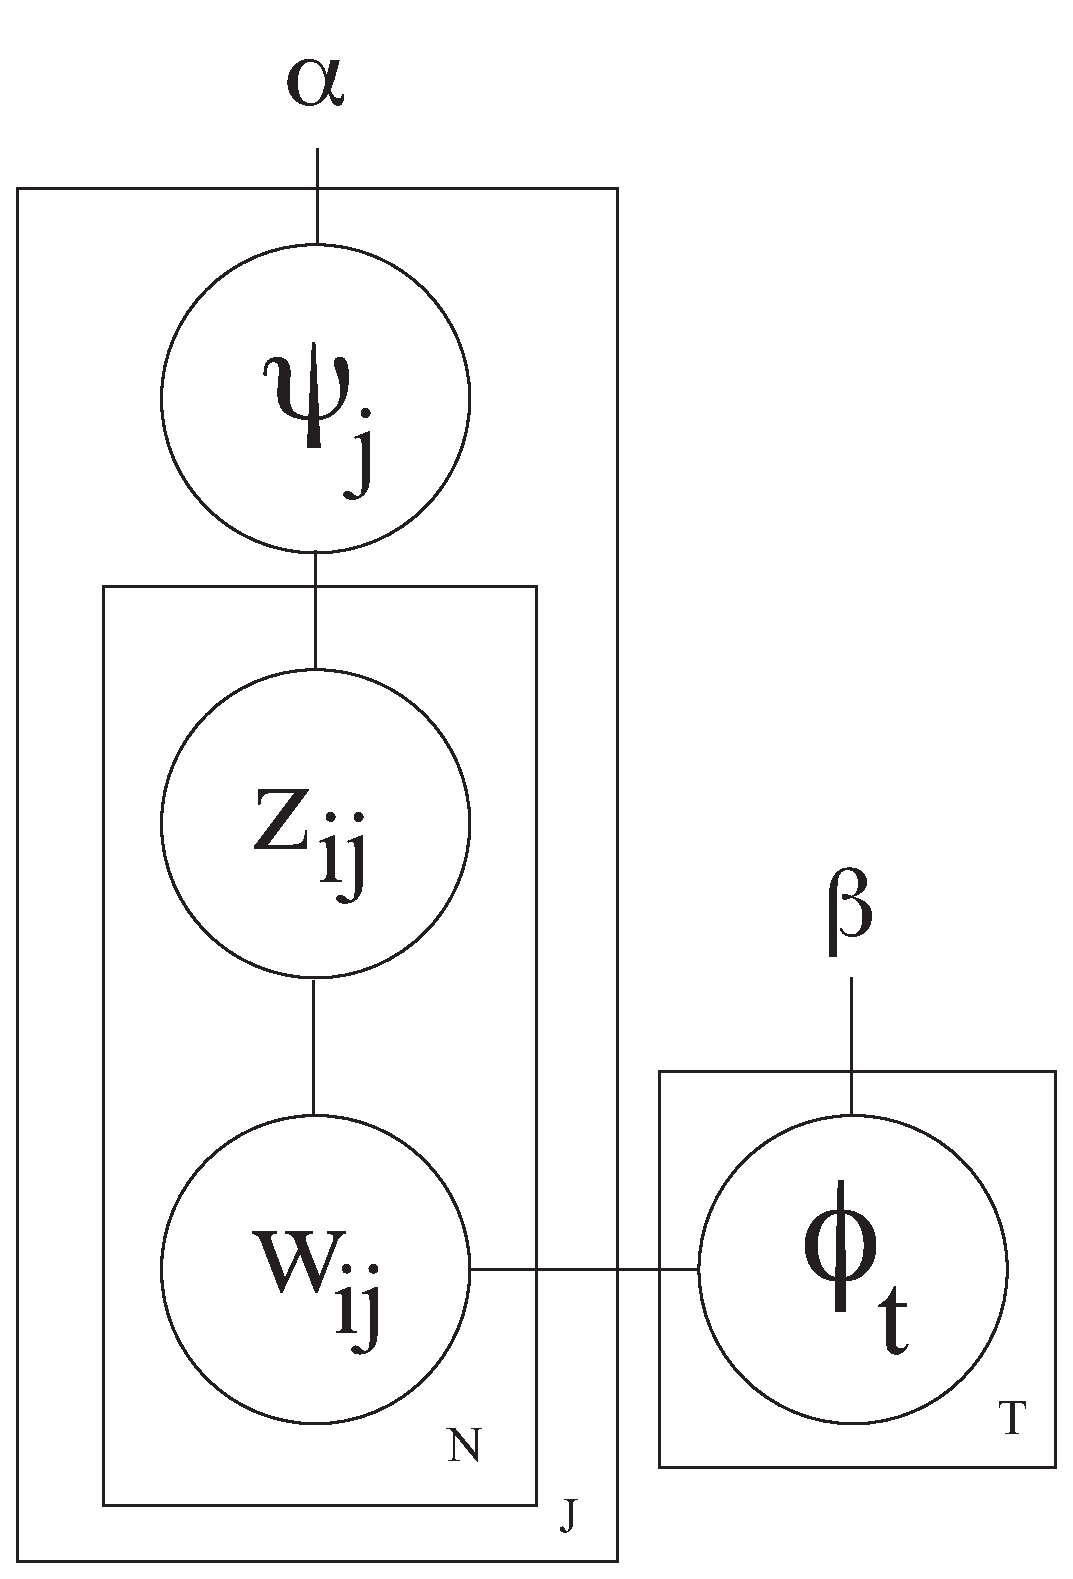
\includegraphics[scale=0.5]{LDA}
%\caption{Graphical Model of Latent Dirichlet Allocation}
%\end{center}
%\end{figure}

%\begin{figure}
%\begin{center}
%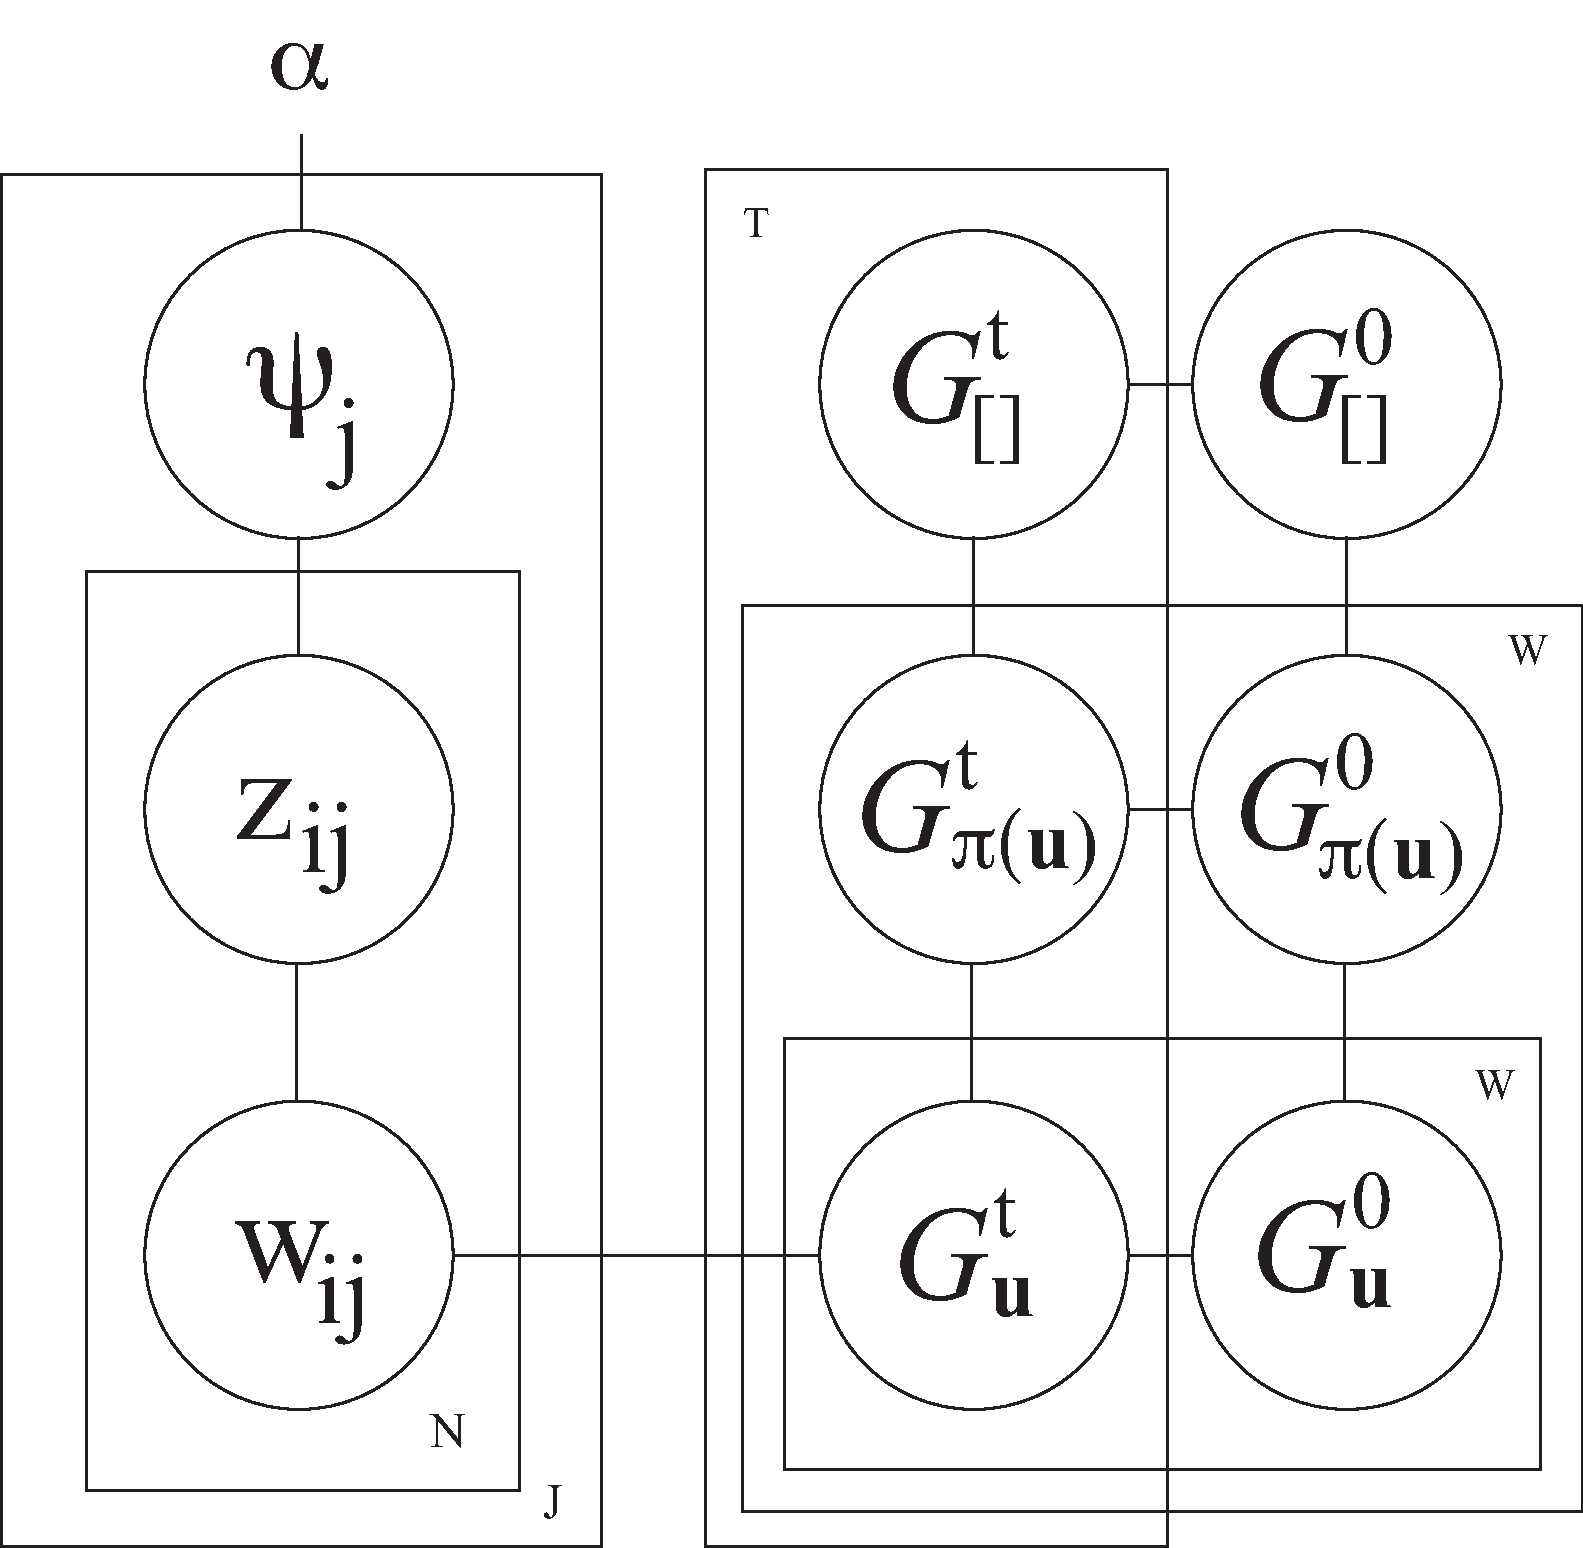
\includegraphics[scale=0.5]{LDA-DHPYPLM2}
%\caption{Graphical Model of LDA-DHPYPLM (excluding hyperparameters)}
%\end{center}
%\end{figure}

\bibliographystyle{latex/acl}
% you bib file should really go here 
\bibliography{../../uber.bib}


\end{document}
